\documentclass{article}

\usepackage{fullpage}
\newcommand{\R}{\proglang{R}}
% For algorithms
\usepackage{algorithm}
\usepackage{algorithmic}

% As of 2011, we use the hyperref package to produce hyperlinks in the
% resulting PDF.  If this breaks your system, please commend out the
% following usepackage line and replace \usepackage{icml2016} with
% \usepackage[nohyperref]{icml2016} above.
\usepackage{hyperref}
\usepackage{xcolor}
\definecolor{Ckt}{HTML}{E41A1C}
\definecolor{Min}{HTML}{4D4D4D}%grey30
%{B3B3B3}%grey70
\definecolor{MinMore}{HTML}{377EB8}
\definecolor{Data}{HTML}{984EA3}

% Packages hyperref and algorithmic misbehave sometimes.  We can fix
% this with the following command.
%\newcommand{\theHalgorithm}{\arabic{algorithm}}

% Employ the following version of the ``usepackage'' statement for
% submitting the draft version of the paper for review.  This will set
% the note in the first column to ``Under review.  Do not distribute.''
%\usepackage{icml2016} 
%\usepackage{fullpage}

% Employ this version of the ``usepackage'' statement after the paper has
% been accepted, when creating the final version.  This will set the
% note in the first column to ``Proceedings of the...''
%\usepackage[accepted]{icml2016}

\usepackage{tikz}
\usetikzlibrary{arrows}
\usepackage{amssymb,amsmath}
\usepackage{natbib}
\usepackage{amsthm}
\newtheorem{proposition}{Proposition}
\newtheorem{lemma}{Lemma}
\newtheorem{theorem}{Theorem}
\newtheorem{definition}{Definition}
\DeclareMathOperator*{\argmin}{arg\,min}
\DeclareMathOperator*{\sign}{sign}
\DeclareMathOperator*{\Lik}{Lik}
\DeclareMathOperator*{\Peaks}{Peaks}
\DeclareMathOperator*{\HotSpots}{HotSpots}
\newcommand{\Cost}{\text{Cost}}
\usepackage{stfloats}
\DeclareMathOperator*{\Diag}{Diag}
\DeclareMathOperator*{\TPR}{TPR}
\DeclareMathOperator*{\Segments}{Segments}
\DeclareMathOperator*{\Changes}{Changes}
\DeclareMathOperator*{\FPR}{FPR}
\DeclareMathOperator*{\argmax}{arg\,max}
\DeclareMathOperator*{\maximize}{maximize}
\DeclareMathOperator*{\minimize}{minimize}
\newcommand{\ZZ}{\mathbb Z}
\newcommand{\NN}{\mathbb N}
\newcommand{\RR}{\mathbb R}


%% -- LaTeX packages and custom commands ---------------------------------------

%% recommended packages
\usepackage{thumbpdf,lmodern}

%% another package (only for this demo article)
\usepackage{framed}

%% new custom commands
\newcommand{\class}[1]{`\code{#1}'}
\newcommand{\fct}[1]{\code{#1()}}


%% -- Article metainformation (author, title, ...) -----------------------------

%% - \author{} with primary affiliation
%% - \Plainauthor{} without affiliations
%% - Separate authors by \And or \AND (in \author) or by comma (in \Plainauthor).
%% - \AND starts a new line, \And does not.
\author{Toby Dylan Hocking}

%% - \title{} in title case
%% - \Plaintitle{} without LaTeX markup (if any)
%% - \Shorttitle{} with LaTeX markup (if any), used as running title
\title{A graph-constrained segmentation model for multi-modal
  regression}

\begin{document}

\maketitle

\begin{figure}
  \centering
  \begin{minipage}{2in}
    \centering
    \textbf{Unconstrained}

    Sparsity in changes

    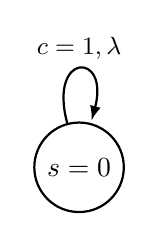
\begin{tikzpicture}[->,>=latex,shorten >=1pt,auto,node distance=2cm,
      thick,main node/.style={circle,draw}]

      \node[main node] (0) {$s=0$};

      \path[every node/.style={font=\sffamily\small}]
      (0) edge [loop above] node {$c=1,\lambda$} (0);
    \end{tikzpicture}
  \end{minipage}
  \begin{minipage}{2in}
    \centering
    \textbf{Up-down constrained}\\
    Sparsity in modes,\\
    One change up to/\\
    down from each mode
    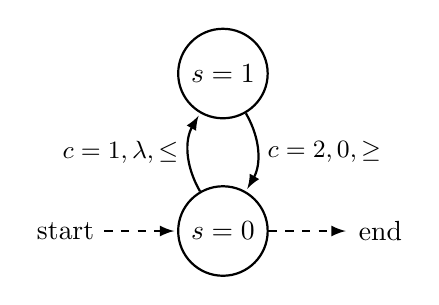
\begin{tikzpicture}[->,>=latex,shorten >=1pt,auto,node distance=2cm,
      thick,main node/.style={circle,draw}]

      \node[main node] (1) {$s=1$};
      \node[main node] (0) [below of=1] {$s=0$};
      \node (start) [left of=0] {start};
      \node (end) [right of=0] {end};

      \path[every node/.style={font=\sffamily\small}]
      (0) edge [bend left] node {$c=1, \lambda, \leq$} (1)
      (start) edge [dashed] (0)
      (0) edge [dashed] (end)
      (1) edge [bend left] node {$c=2, 0, \geq$} (0);
    \end{tikzpicture}
  \end{minipage}
  \begin{minipage}{2in}
    \centering
    \textbf{Asymmetric multi-modal regression}\\
    Sparsity in modes,\\
    Many changes up to/\\
    down from each mode
    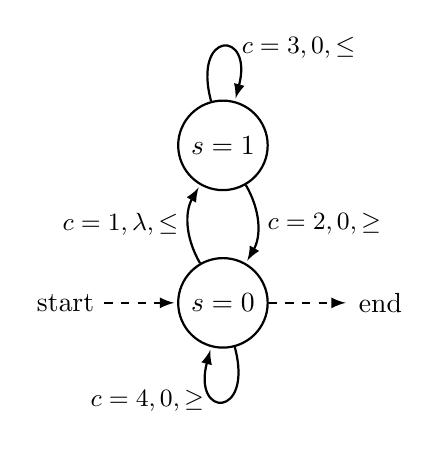
\begin{tikzpicture}[->,>=latex,shorten >=1pt,auto,node distance=2cm,
      thick,main node/.style={circle,draw}]

      \node[main node] (1) {$s=1$};
      \node[main node] (0) [below of=1] {$s=0$};
      \node (start) [left of=0] {start};
      \node (end) [right of=0] {end};

      \path[every node/.style={font=\sffamily\small}]
      (0) edge [bend left] node {$c=1, \lambda, \leq$} (1)
      (start) edge [dashed] (0)
      (0) edge [dashed] (end)
      (0) edge [loop below] node [left] {$c=4,0,\geq$\ \ } (0)
      (1) edge [loop above] node [right] {\ $c=3,0,\leq$} (1)
      (1) edge [bend left] node {$c=2, 0, \geq$} (0);
    \end{tikzpicture}
  \end{minipage}
  \caption{State graphs for three changepoint models. Nodes represent
    states and solid edges represent changepoints. \textbf{Left:} in
    this context, the classical unconstrained optimal changepoint
    model can be represented by the graph with one node and one
    looping edge with penalty $\lambda$. \textbf{Middle:}
    non-decreasing changes $c=1$ to each mode $s=1$ must be followed
    by non-increasing changes $c=2$ to the background state $s=0$, and
    vice versa. \textbf{Right:} our preliminary code for multi-modal
    regression adds a looping edge for each state; these allow
    un-penalized changes up to/down from each mode.}
  \label{fig:state-graph}
\end{figure}

For genomic data such as ChIP-seq \citep{chip-seq}, it is desirable to
have a changepoint model which is interpretable in terms of peaks
(large values) and background noise (small values). It is also
desirable for the model to predict the precise locations of peak
summits (the largest value). We therefore propose a new multi-modal
regression model which is capable of identifying peak summits, based
on the constraint graph shown in Figure~\ref{fig:state-graph},
right. We have previous described a functional pruning algorithm which
can be used to compute the optimal solution for a given penalty
$\lambda$ parameter \citep{Hocking-constrained-changepoint-detection}.

\begin{figure}
  \centering
  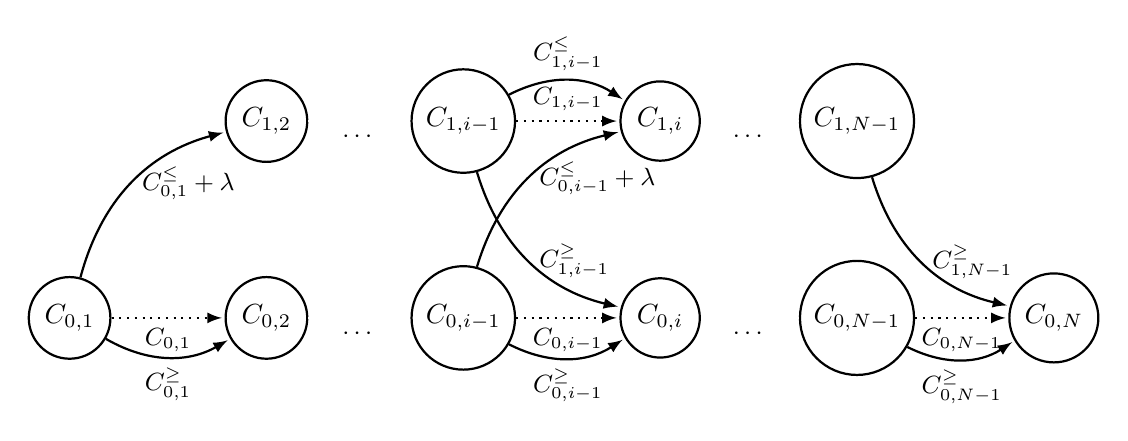
\begin{tikzpicture}[->,>=latex,shorten >=1pt,auto,node distance=2.5cm,
    thick,main node/.style={circle,draw}]
    \node[main node] (peak_t1) {$ C_{1,i-1}$};
    \node[main node] (bkg_t1) [below of=peak_t1] {$ C_{0,i-1}$};
    \node[main node] (peak_t) [right of=peak_t1] {$ C_{1,i}$};
    \node[main node] (bkg_t) [right of=bkg_t1] {$ C_{0,i}$};
    \node[main node] (peak_2) [left of=peak_t1] {$ C_{1,2}$};
    \node[main node] (bkg_2) [left of=bkg_t1] {$ C_{0,2}$};
    \node[main node] (peak_N1) [right of=peak_t] {$ C_{1,N-1}$};
    \node[main node] (bkg_N1) [right of=bkg_t] {$ C_{0,N-1}$};
    \node[main node] (bkg_N) [right of=bkg_N1] {$ C_{0,N}$};
    \node[main node] (bkg_1) [left of=bkg_2] {$ C_{0,1}$};
    \path[every node/.style={font=\small}]
    (peak_t1) edge [dotted] node {$ C_{1,i-1}$} (peak_t)
    (peak_t1) edge [black, bend right] node [right] {$ C_{1,i-1}^{\geq}$} (bkg_t)
    (bkg_t1) edge [dotted] node[midway, below] {$ C_{0,i-1}$} (bkg_t)
    (bkg_t1) edge [black, bend left] node[right] {$ C_{0,i-1}^{\leq}+\lambda$} (peak_t)
    (bkg_1) edge [black, bend left] node[right] {$ C_{0,1}^{\leq}+\lambda$} (peak_2)
    (bkg_1) edge [dotted] node[midway, below] {$ C_{0,1}$} (bkg_2)
    (peak_N1) edge [black, bend right] node [right] {$ C_{1,N-1}^{\geq}$} (bkg_N)
    (bkg_N1) edge [dotted] node[midway, below] {$ C_{0,N-1}$} (bkg_N)
    (bkg_2) edge [color=white] node[below, text=black, pos=0.5] {$\cdots$} (bkg_t1)
    (peak_2) edge [color=white] node[below, text=black, pos=0.5] {$\cdots$} (peak_t1)
    (bkg_N1) edge [color=white] node[below, text=black, pos=0.5] {$\cdots$} (bkg_t)
    (peak_N1) edge [color=white] node[below, text=black, pos=0.5] {$\cdots$} (peak_t)
    (bkg_1) edge [black, bend right] node[below] {$C_{0,1}^\geq$} (bkg_2)
    (bkg_N1) edge [black, bend right] node[below] {$C_{0,N-1}^\geq$} (bkg_N)
    (bkg_t1) edge [black, bend right] node[below] {$C_{0,i-1}^\geq$} (bkg_t)
    (peak_t1) edge [black, bend left] node[above] {$C_{1,i-1}^\leq$} (peak_t)
    ;
  \end{tikzpicture}
  \caption{Directed acyclic graph (DAG) representing dynamic
    programming computations for our preliminary implementation of the
    asymmetric multi-modal regression model. Nodes in the graph repesent cost
    functions, and edges represent inputs to the the pointwise
    $\min\{\}$ operation (solid=changepoint, dotted=no change). There
    is one column for each data point and one row for each state: the
    optimal cost of the increasing state $s=1$ at data point $i$ is
    $ C_{1,i}$ (top row); the optimal cost of the decreasing
    state $s=0$ is $ C_{0,i}$ (bottom row).}
  \label{fig:computation-graph}
\end{figure}

% \begin{figure}
%   \centering
%   \begin{tikzpicture}[->,>=latex,shorten >=1pt,auto,node distance=2.5cm,
%     thick,main node/.style={circle,draw}]
%     \node[main node] (peak_t1) {$ C_{1,i-1}$};
%     \node[main node] (bkg_t1) [below of=peak_t1] {$ C_{0,i-1}$};
%     \node[main node] (peak_t) [right of=peak_t1] {$ C_{1,i}$};
%     \node[main node] (bkg_t) [right of=bkg_t1] {$ C_{0,i}$};
%     \path[every node/.style={font=\small}]
%     (peak_t1) edge [dotted] node {$ C_{1,i-1}$} (peak_t)
%     (peak_t1) edge [black, bend right] node [right] {$ C_{1,i-1}^{\geq}$} (bkg_t)
%     (bkg_t1) edge [dotted] node[midway, below] {$ C_{0,i-1}$} (bkg_t)
%     (bkg_t1) edge [black, bend left] node[right] {$ C_{0,i-1}^{\leq}+\lambda$} (peak_t)
%     (bkg_t1) edge [black, bend right] node[below] {$C_{0,i-1}^\geq$} (bkg_t)
%     (peak_t1) edge [black, bend left] node[above] {$C_{1,i-1}^\leq$} (peak_t)
%     ;
%   \end{tikzpicture}
%   \caption{Directed acyclic graph (DAG) representing dynamic
%     programming computations for the
%     symmetric multi-modal regression model. }
%   \label{fig:computation-graph}
% \end{figure}

\begin{figure}
  \centering
  \includegraphics[width=\textwidth]{figure-Mono27ac-label-error-zoom}
  \caption{Our previously proposed labeling method and databases can
    be used to train the new multi-modal regression model, by
    selecting a penalty that minimizes the number of label
    errors. \textbf{Top:} penalty=500 results in two false positive
    noPeaks labels which should have no predicted peak summits (green
    dots). \textbf{Bottom:} penalty=50000 results in a false negative
    peakStart label which should have exactly one run of increasing
    segments. \textbf{Middle:} penalty=3000 results in zero label
    errors so is a good fit for these data.}
  \label{fig:label-error}
\end{figure}

% \begin{figure}
%   \centering
%   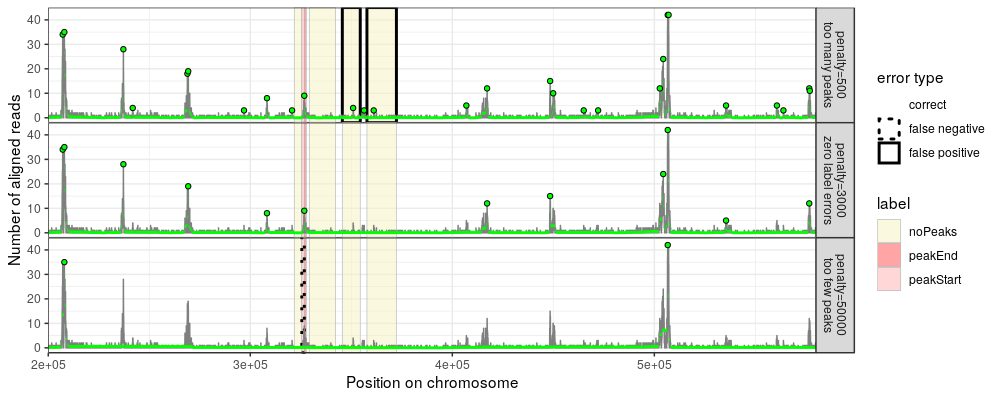
\includegraphics[width=\textwidth]{figure-Mono27ac-label-error}
%   \caption{Zooming out shows a larger portion of the data in which the algorithm has been used to detect peak summits using three different penalty parameters.}
%   \label{fig:zoom-out}
% \end{figure}
%\includegraphics[width=\textwidth]{figure-Mono27ac-label-error-zoom2}

\begin{figure}
  \centering
  \includegraphics[width=\textwidth]{figure-Mono27ac-summits-vs-peaks}
  \caption{Two models with 10 peaks but with different graph-based
    constraints. \textbf{Top:} Previous model with two edges enforces
    a non-increasing change after each non-decreasing change (and vice
    versa) results in one segment per peak. It misses a labeled peak
    (false negative purple rectangle) and predicts an unwanted peak
    (false positive yellow rectangle). \textbf{Bottom:} Proposed model
    with four edges allows several non-decreasing changes up to a peak
    summit, followed by several non-increasing changes down to
    background noise.}
  \label{fig:summits-vs-peaks}
\end{figure}

\begin{figure}
  \centering
  \includegraphics[width=\textwidth]{figure-AR1-multimodal.png}
  \caption{Two models for neuro spike train data. \textbf{Left:} In
    these data the previously proposed AR1 model misses a spike in the
    left label (false negative) and predicts two spikes where there
    should be only one in the right label (false
    positive). \textbf{Right:} The proposed multimodal regression
    model correctly detects the spikes in the left and right labels.}
  \label{fig:AR1-multimodal}
\end{figure}

\bibliographystyle{abbrvnat}
\bibliography{refs}

\end{document}
\